
\chapter{语音识别中的解码搜索问题}
\label{chap:intro2}

本章中,我们首先介绍基本的维特比解码搜索算法,而后引入其在语音识别中的应用。我们对语音识别中的解码搜索问题及其当前解决方案进行了详细介绍。这些不同的技术流派包括同步和非同步之分,以及动态和静态之分。我们对近十年主流的加权有限状态机技术进行了重点介绍。基于上面的介绍,我们总结了当前解码器研究中的待解决问题,以及上一章中深度序列学习模型所带来的研究机遇。后续本论文的一系列工作将基于本章针对解码器的分析,讨论和总结。


\section{维特比解码搜索算法}
\label{chap:intro2-viterbi}

维特比算法是一种动态规划算法,用于寻找维特比路径,其对应于最有可能产生观测事件的序列,即隐含状态序列。这一算法最早由安德鲁·维特比(Andrew Viterbi)在1967年提出,用于在数字通信链路中解卷积以消除噪音。 此算法被广泛应用于GSM和CDMA数字蜂窝网络、拨号调制解调器、深空通信、卫星和802.11无线网络中的解卷积码。另一大类应用为计算语言学和生物信息学,以及语音识别和关键字检测。例如在语音识别中,声音信号作为观察到的事件序列,而文本字符串,被看作是隐含的产生声音信号的给定原因,因此可对声音信号应用维特比解码搜索算法寻找最有可能的文本字符串序列。

假设给定隐式马尔可夫模型(HMM)状态空间 S, 初始处于状态i 的概率 $\pi_{i}$ 以及转移概率 $a_{i,j}$,其对应于从状态i转移到状态j的概率。同时我们观测到输出序列 $y_{1},\dots ,y_{T}$。 其对应的产生该观察序列的相应隐状态 $x_{1},\dots ,x_{T}$ 可以由递推关系得到。

\begin{equation}
\begin{split}
V_{1,k}=\mathrm {P} {\big (}y_{1}\ |\ k{\big )}\cdot \pi _{k}
\end{split}
\end{equation}
\begin{equation}
\begin{split}
V_{t,k}=\max _{x\in S}\left(\mathrm {P} {\big (}y_{t}\ |\ k{\big )}\cdot a_{x,k}\cdot V_{t-1,x}\right)
\end{split}
\end{equation}

\begin{equation}
\begin{split}
V_{1,k}=\mathrm {P} {\big (}y_{1}\ |\ k{\big )}\cdot \pi _{k}
\end{split}
\end{equation}
\begin{equation}
\begin{split}
V_{t,k}=\max _{x\in S}\left(\mathrm {P} {\big (}y_{t}\ |\ k{\big )}\cdot a_{x,k}\cdot V_{t-1,x}\right)
\end{split}
\end{equation}

这里的$V_{t,k}$表示前 t 个最终状态为 k 的观测结果最有可能对应的状态序列的概率。通过保存向后指针记住在第二个等式中用到的状态 x 可以获得维特比路径。声明一个函数$\mathrm {Ptr} (x_{t},t)$ ,它返回若 $t>1$ 时计算 $V_{t,k}$ 用到的 x 值 或若 $t=1$ 时的 k,这样:


\begin{equation}
\begin{split}
x_{T}=\arg \max_{x\in S}(V_{T,x})
\end{split}
\end{equation}
\begin{equation}
\begin{split}
x_{t-1}=\mathrm {Ptr} (x_{t},t)
\end{split}
\end{equation}
\begin{equation}
\begin{split}
x_{T}=\arg \max _{x\in S}(V_{T,x})
\end{split}
\end{equation}
\begin{equation}
\begin{split}
x_{t-1}=\mathrm {Ptr} (x_{t},t)
\end{split}
\end{equation}

这里我们使用了arg max的标准定义,算法复杂度为 $O(T\times \left|{S}\right|^{2})$。一个更好的估计存在于迭代只针对那些可以连接到当前状态的下一个状态当中,那么算法复杂度为 $O(T\times (\left|{S}\right|+\left|{E}\right|))$,其中的E 表示图中所存在的边数。

\section{语音识别中的解码搜索问题}
\label{chap:intro-asr-dec}

语音信号的识别既是一个模式识别问题,也包含相应的推理搜索问题。前一个问题对各种语音信号的、语言现象进行数学表示和描述,在基于统计学习的模式识别框架下进行建模,这决定了语音信号的识别系统可达到识别准确度的上限。而后一个问题在给定模型情况底下,研究如何高效地将输入语音信号的和模型相匹配,推理搜索得到最优识别结果,这决定了识别速度和实际可达的识别准确度。
在语音信号的识别的推理搜索阶段,解码器功能是对声学模型计算出的声学特征概率和语言模型计算出的语言概率进行组合来得到最大概率的词序列。

在语音识别中,声音信号作为观察到的事件序列,而文本字符串,被看作是隐含的产生声音信号的给定原因,因此可对声音信号应用维特比解码搜索算法寻找最有可能的文本字符串序列,称为语音识别的推理搜索阶段。
%
在语音信号的识别推理搜索阶段,解码器是语音信号的识别系统的核心和灵魂,所有信息都汇集于此。它将不同来源、 不同层次、 不同性质的知识和信息关联在一起,使它们互相之间取长补短, 从而得到正确的语音信号的识别结果。因此,如何将各种性质不同的信息有机融合是解码网络和解码算法设计中必须认真研究和解决的重要问题之一。
从解码器的作用来看,它不仅是验证语音信号识别中各种理论,模型和算法正确性的基本实验平台,也是构建实际系统的基础。因此,在解码器设计中,还必须考虑到研究的便利性和工程的实际应用。

语音识别系统可以分为关键词检测,孤立词识别,语法网络识别,大词汇连续语音识别和基于神经网络语音模型的大词汇连续语音识别,下面我们将对它们中的解码搜索问题进行逐一介绍。

\subsection{关键词检测和孤立词识别}
\label{chap:intro-kws-dec}

%综述关键词检测
关键词检测(KWS)是语言识别最主要的应用之一,它的目标是得到一个高准确度和高效率的识别器,用于检测特定的一些关键词在语音中的出现。
KWS可以被用于声学数据挖掘~\cite{zhou2005data}, 低资源的音频检索~\cite{shen2009comparison}, 
语料库检索~\cite{garofolo2000trec} 和 唤醒词识别~\cite{chen2014small}。

KWS 技术可以被分为两大类:
i) 非监督的  {\em query-by-example} (QbyE) \cite{zhang2009unsupervised,barakat2012improved,chen2015query}, 它使用了关键词的声学样例来产生一系列模板,之后尝试将模板与测试音频样例进行匹配来决定是否被唤醒。
ii) 监督的基于文本的方法,这部分可以被进一步分类为  基于{\em 大词汇连续语音识别} (LVCSR)  方法 ~\cite{garofolo2000trec,ng2000subword} 和  {\em 声学 KWS} \cite{mandal2014recent}。
对于前者,在训练阶段需要构建一个词,半词或音素的语音识别系统。声学和语言模型在测试阶段一起对语音进行转录并得到词图。之后在词图上进行关键词搜索得到最终的结果。
声学 KWS 不需要语言模型,通过直接建模目标关键词,半词或音素,构建一个声学模型来进行关键词的判别。一些方法中也会考虑引入非关键词元素到建模当中~\cite{sukkar1996utterance}。
QbyE 主要用于低资源音频检索, 本文不针对这个方向。 
在 语料库检索中, 基于LVCSR方法通常能得到更好的性能,相比声学KWS。但是基于LVCSR方法也有如下一些缺点: 需要训练一个非常通用的大词汇连续语音识别系统,因此需要大量语料;同时在测试阶段也需要非常大的词表进行覆盖。这样的缺点限制了它在一些应用,比如唤醒词识别中的应用。除此之外,基于LVCSR的方法忽略了KWS任务本身的一些特性,该类方法的推理搜索阶段解码搜索算法主与大词汇连续语音识别中类似,详细讨论参加下一章节。

在声学关键词检测中,模型通常是进行逐帧分类的。解码方法用于解决模型所造成的误唤醒问题。解码的搜索空间通常包含两个部分:领域内搜索空间和领域外搜索空间。前者由关键词序列得到,而后者通常可以由特定模型进行建模(比如后文将提到的$filler$模型)领域外的搜索空间。另一方面如果KWS建模不是直接针对关键词,而是针对关键词的子序列,则搜索空间还需要建模子序列与目标关键词之间的映射关系(比如词典和发音序列)。

%综述孤立词识别
孤立词识别是指对用户单个词语孤立发音的语音识别。
在特定人孤立词语音识别中,最为简单有效的方法是采用动态时间规整(Dynamic Time Warping,DTW) 算法,该算法基于动态规划的思想,解决了语音长短不一的模板匹配方面的问题,是语音识别中出现最早且较为经典的一类算法。这类算法依然基于动态规划和维特比搜索解码。DTW通过把时间序列进行延伸和缩短,来计算两个时间序列性之间的相似性。其计算遵循一定的搜索规则,根据语音信号在时间上的连贯性,认为所有路径均是从第一帧出发,并在最后一帧和最后一个输出上结束。由于两序列之间不等长,所以需要在匹配过程中限定弯折率来实现。最优路径为在满足约束条件下,计算路径累计距离的最小值。



\subsection{语法网络识别和大词汇连续语音识别}
\label{chap:intro-lvcsr}

%语法网络
孤立词的语音并不是人类沟通的自然方式。为了建模人类的自然语言,一种方法是使用语法网络来进行语音识别。
语法网络可以规定词语按照什么规则来合成句子,即概率式句法结构。
在该网络中,每个句子由若干词条组成,每一个词条都选自词汇表。句子中一个要选择的词条以一定的概率出现,而选择第二个词条的概率与前一个词条出现的概率有关,以此类推,直到句子的结束。在此框架里,每一个词语由若干个音素串接而成。而后每一个音素用一个HMM模型以及一套参数来表示。每一个HMM模型中最基本的构成单位是状态与状态之间的转移弧以及每个状态的概率建模。这样,从HMM状态出发逐层扩大到音素、词语、句子。每一个句子是包含许多状态的复杂的状态图,该句子就是用所有状态形成的结构、状态之间的转移概率,以及每个转移弧产生某个特征输出的概率来描述。对于特定的词表和句法,所有可能出现的句子构成一个更大的状态图。在完成识别任务的时候,要根据一个输入语音特征矢量序列来确定一个最可能的句子。这就需要在这个大的状态图中搜索一条路径,该路径上产生上述特征矢量的概率最大,有路径可以进一步确定句子中的每一个词。这种路径搜索就是采用维特比搜索算法。

语音识别中更具有挑战性的研究课题则是大词汇量、非特定人的连续语音识别,称为大词汇连续语音识别。
大词连续语音识别中,语音信号先经过分析后形成特征矢量,并按隐马尔科夫模型,上下文音素,字典和词模型,语言模型结合而成的搜索空间进行识别,最后得到相应的句子。

与关键词检测和孤立词识别相比:传统语音识别模型要针对整个短语序列进行识别显然是不可能的,因为语言中短语的数量太多,所以必须把输入的语流切分为更小的组分来进行,相比较人类感知语音的过程也是类似的。由于连续语音中间没有间歇,所以在识别前必须先把各字拆分开,这就需要系统必须能够识别单词之间的边界关系。但这是非常困难的,因为确定单词间的边界位置还没有现成的方法来进行。尽管有时候可以采用能量最低点作为边界的判断准则,但是通常要根据发音信息加以辅助验证。另一方面,连续语音的发音比孤立词的发音跟随便,受协同发音的影响也就更为严重。除此之外,连续语音识别系统中的很多问题都与相应的语言学知识有关,特别是大词汇连续语音识别系统要更多地强调运用语言学知识来进行。

另一方面,大词汇连续语音识别的解码过程复杂度非常高。解码搜索的复杂度与上述由隐马尔科夫模型一直到语言模型的各个层面相关。下面我们将举例子进行说明。
%在语音识别里搜索意味什么,词级,语法级,语言模型,神经网络级(search基本形态); 为什么难,复杂度多高;
首先在有限状态语法网络网络以及 unigram和monophone情况下,其语法网络如图~\ref{fig:exp-ug}所示。
该语法网络在每帧上的近似的复杂度包括两部分:
\begin{enumerate}
\item 内部传递: $W_{\tt ug}\times P\times N$, 其中 $P$ 是每个词的平均音素数量, $N$ 是每个模型的状态个数
\item 外部传递: $W_{\tt ug}\times P + W_{\tt ug}$ 
\end{enumerate}
而扩展到unigram的情况,在每一个词的开始,将unigram的概率加到令牌的对数似然度上,使得语言模型的信息尽可能早地合并进来。

\begin{figure}[!htp]
  \centering
    \captionstyle{\centering}
    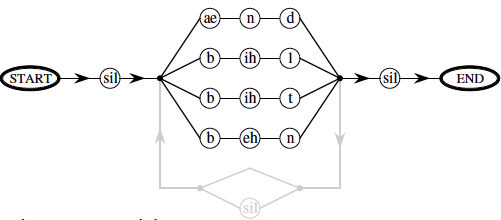
\includegraphics[clip=true, width=\textwidth]{figure/ug.png}
    \bicaption[fig:exp-ug]{}{有限状态语法网络网络以及 unigram和monophone}{Fig}{Finite State Grammar Newwork with unigram and monophone}
\end{figure}

而如果扩展到Bigram和monophone情况下,其语法网络如图~\ref{fig:exp-bg}所示。在每帧上的近似的复杂度则包括内部传递: $W_{\tt ug}\times (P+1)\times N$ 和 外部传递: $W_{\tt ug}\times P + W_{\tt ug}^2$。而如果使用回退back-off语言模型, 词传递大致是 $W_{\tt bg}+W_{\tt bo}\times W_{\tt ug}$。

\begin{figure}[!htp]
  \centering
    \captionstyle{\centering}
    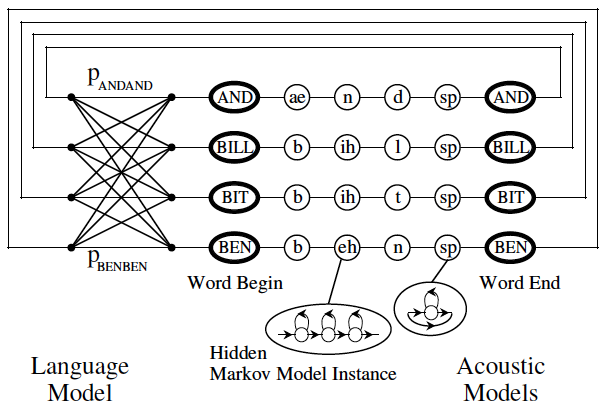
\includegraphics[clip=true, width=\textwidth]{figure/bg.png}
    \bicaption[fig:exp-bg]{}{Bigram和monophone的语法网络}{Fig}{Finite State Grammar Newwork with Bigram and monophone}
\end{figure}


再扩展到Bigram和cross-word triphone 情况下,其语法网络如图~\ref{fig:exp-xwrdbg}所示。在每帧上的近似的复杂度则包括内部传递: $W_{\tt ug}\times (P-2+ P_{\tt prefix}+ P_{\tt suffix})\times N$ 和 外部传递: $W_{\tt ug}^2 + W_{\tt ug}\times (P-2+ P_{\tt prefix}+ P_{\tt suffix})$。

\begin{figure}[!htp]
  \centering
    \captionstyle{\centering}
    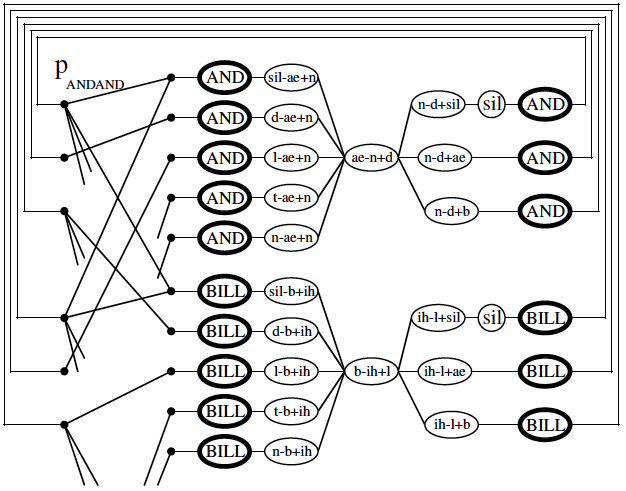
\includegraphics[clip=true, width=\textwidth]{figure/xwrdbg.png}
    \bicaption[fig:exp-xwrdbg]{}{Bigram和cross-word triphone的语法网络}{Fig}{Finite State Grammar Newwork with Bigram and cross-word triphone}
\end{figure}

如果使用Trigram和within-word triphone,其语法网络如图~\ref{fig:exp-tg}所示。在每帧上的近似的复杂度则包括内部传递: $W_{\tt ug}^2\times (P+1)\times N$ 和 外部传递: $W_{\tt ug}^3 + W_{\tt ug}^2\times (P+1)$。
如果是回退back-off LM, 词传递大致是$W_{\tt tg}+W_{\tt bo}^{\tt bg}(W_{\tt bg}+W_{\tt bo}W_{\tt ug}) $。

目前业界最主流的系统使用trigram语言模型和跨词三音子triphone声学模型,该情况下,解码复杂度会变得甚至更大。因此在下一章节中我们将介绍如何在复杂度如此之高的搜索网络上进行解码搜索。

\begin{figure}[!htp]
  \centering
    \captionstyle{\centering}
    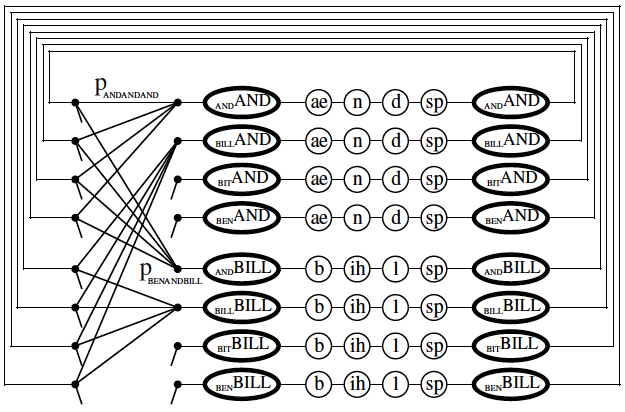
\includegraphics[clip=true, width=\textwidth]{figure/tg.png}
    \bicaption[fig:exp-tg]{}{Trigram和within-word triphone的语法网络}{Fig}{Finite State Grammar Newwork with Trigram and within-word triphone}
\end{figure}

\section{解码器技术综述}
\label{chap:intro2-dec-sum}

\subsection{解码器的技术流派}
\label{chap:intro-lvcsr-decmethod}

\subsubsection{静态和动态的搜索空间构建方法}
\label{chap:intro-lvcsr-decmethod-graph}

根据前面章节讨论,完整的语音信号识别系统由自下而上的五层映射关系组成:语音信号到HMM状态的观察,HMM状态到依赖于上下文的音素,依赖于上下文的音素到音素,音素到单词,单词到句子。
具体来说公式~\ref{eq:decode}可以进一步展开如下:
\begin{equation}
 \begin{split}
\mathbf{w}^* = \arg \max_{\mathbf{w} \in \mathcal{H}} \max_{\mathbf{s}} P(\mathbf{s}|\mathbf{w})p(\mathbf{O}|\mathbf{s})P(\mathbf{w}) \\
= \arg \max_{\mathbf{w}} \sum_{\mathbf{l}} \sum_{\mathbf{c}} \sum_{\mathbf{s}}
p(\mathbf{O}|\mathbf{s}) \cdot
P(\mathbf{s}|\mathbf{c})\cdot P(\mathbf{c}|\mathbf{l})\cdot P(\mathbf{l}|\mathbf{w}) \cdot 
P(\mathbf{w})
 \end{split}
\end{equation}
其中展开后式子每一项分别对应上述的五层映射关系。
在识别之前不能知道语音信号的观察,因此需要在解码过程中动态地建立观察到的语音信号的HMM状态的映射,并且还需要实时计算相应的声学分数。对于从HMM状态到依赖于上下文的音素,依赖于上下文的音素到音素,音素到单词的三级映射关系,一旦确定了发音字典和声学模型,它们就不会改变。为了追求解码效率,人们通常将它们静态编译成解码网络。对于没有任何约束的大词汇量连续语音信号的识别任务,可以以任何方式将单词组织成句子,因此原则上,单词 - 句子映射关系只能在解码过程中动态建立。然而,由于表征单词和单词之间的关联度(概率)的N-gram语法模型在解码之前已经存在并且是有限集,因此在实践中,语言模型得分计算可以以不同方式实现。在语音信号识别领域,根据解码器中语言模型的表示,语言模型状态获取和语言模型得分计算方法,解码器通常分为两大流派:
\begin{itemize}
\item 动态网络解码器: 在动态网络解码器中,解码网络仅包含发音字典和声学
模型,不会含有语言模型任何信息。 语言模型状态在解码过程中还要随着词与词相连
成句而动态地生成、语言模型分数通过去查表的方式动态地获取。这类解码器的典型
代表是基于发音前缀树(Pronunciation Prefix Tree, PPT)~\cite{woodland1994large}网络解码器。
\item 静态网络解码器: 在静态网络解码器中,解码网络不仅包含发音字典和声
学模型,也包含完整的语言模型分数。 语言模型状态以及状态转移以WFST的形
式合成到解码网络中去, 语言模型分数则作为状态转移概率存储于边上。解码时,
仅需逐边积累整条路径状态转移概率便可获得语言模型分数。这类解码器的典
型代表是基于加权有限状态转换器(WFST)~\cite{mohri2002weighted}的解码器。
\end{itemize}

作为一种时空变换策略,静态网络解码器通常可以通过仔细优化实现更快的识别速度,但缺点是显而易见的:构建的解码网络太大,特别是在高阶语言中。在模型和声学模型的情况下,由于存储器大小限制,将所有知识源编译到解码网络中通常是不可行的。因此,近年来,基于动态解码网络的传统解码信号的识别方法逐渐受到研究者的青睐~\cite{soltau2009dynamic,rybach2011comparative}, 能够几乎不受任何约束地利用更高阶语言模型和声学模型以便获得更优异的识别准确度, 应用面更广, 这是动态网络解码器最为吸引人的地方。然而动态网络解码器的设计和束搜索剪枝方法更加复杂,需要调整参数和阈值更多,挑战性更大。 

\subsubsection{同步和异步的搜索算法}
\label{chap:intro-lvcsr-decmethod-search}

除了根据解码网络的结构进行分类之外,还可以根据搜索最优路径的不同方式将解码器划分为时间异步搜索解码器和时间同步搜索解码器:

\begin{itemize}
\item 时间异步搜索解码器: 在较老的解码器,例如: IBM ViaVoice 中, 采用深度优先方式在解码网络中搜索最优词序列, 是一种时间异步搜索。由于这类解码
器在解码过程中需要用到一些后进先出的缓冲区(即:堆栈)来保存扩展得到词识别假设,所以也常常被称为堆栈解码器(Stack decoder)~\cite{paul1992efficient}。 
与时间同步搜索相比,优点在于通过选择适当的启发函数,搜索可以控制于最佳路径附近,并且提高了搜索效率。但这也造成了它的主要缺陷:1)启发函数综合声学和语言分数,有时需要“未来”路径信息,因此很难获得; 2)因为它是时间异步搜索,所以搜索过程产生的路径长度各不相同,使得修剪很难实现。因此,当前的堆栈解码很少用于直接解码语音信号的观察,而更多地用作用于从字图生成N-Best结果的后处理中。
\item 时间同步搜索解码器:时间同步搜索是目前解码器设计和实现的主流方法,也称为帧同步搜索。它使用广度优先方法找到与来自解码网络的输入特征序列最佳匹配的状态序列,以便获得相应的最佳音素序列和字序列。这种类型的解码器通常使用维特比算法或令牌传递算法~\cite{woodland1994large}实现。 
\end{itemize}

时间异步的搜索算法还包括多遍解码算法。多遍解码算法通常在每次解码过程中对之前的搜索空间进行剪枝,缩小空间大小,而后将压缩后的搜索空间交给下一次解码算法,进行进一步搜索,直到最终得到最佳结果。
为在搜索中利用各种各样的知识源,通常要进行多遍搜索,第一遍要使用代价较低的知识源,产生一个候选序列列表或词候选网格,在此基础上再进一步进行使用代价高的知识源的第二遍搜索来得到最佳路径。这里的知识源包括声学模型、语言模型和音标词典,这些可以用于第一遍搜索。为实现更准确的语音识别,往往要利用一些代价更高的知识源,如高阶的上下文相关的N-Gram语音模型、词间混淆相关模型、分段模型或语法分析算法,进行重新打分。目前主流的实时大词汇连续语音识别系统许多都使用这种多遍搜索策略。
与单遍搜索(1-pass)相比,多遍搜索具有优点和缺点,并且它也在实践中使用。多遍搜索的支持者认为:第一遍粗搜索可以大大减少解码空间,使得在后续解码过程中使用更精细的语言模型和声学模型成为可能,避免了单遍解码器中的时间和空间限制。 。单遍搜索的支持者认为在多遍解码中存在三个主要问题:1)由于第二遍解码必须等待第一遍解码,因此多遍搜索难以应用于实时解码。 2)每次通过解码引入了不可恢复的修剪误差,其不能被后续解码中使用的任何模型补偿。要解决这个问题,我们仍然需要努力研究单遍搜索算法。最好直接进行单遍解码器。 3)多次解码器的每次解码中使用的特征,声学模型,语言模型和搜索算法是不同的。

解码器不仅算法复杂,而且需要高工程能力和技能。在开发完成后,通常需要大量的人力和时间进行调整。因此,各种研究机构和商业公司都有自己的解码器实现细节。它就像它一样深。尽管如此,世界上仍有一些用于学术研究的开源解码器可以作为研究的基础。该表列出了比较知名的那些。这些解码器的网络结构和解码算法不同,但由于学术研究的目的,大多数速度优化都比较差。


\begin{table}[thbp!]
  \caption{\label{tab:perf-compare} {\it  知名开源解码器 } }
  \centerline{
    \begin{tabular}{c c  c c}
      \toprule
      解码器 &  研发机构 & 网络结构 & 搜索算法 \\
      \midrule
      HDecode & 英国剑桥大学 & 动态,发音前缀树 & 单遍, 令牌传递 \\
        Sphinx &美国卡内基梅隆大学 &动态,发音前缀树 &单遍, 令牌传递 \\
        RASR &德国亚琛工业大学& 动态, 发音前缀树 &单遍, Viterbi \\
        Juilus & 日本京都大学 & 动态, 发音前缀树 & 两遍, 前后向搜索。\\
        Juicer & 瑞士IDIAP & 静态, WFST & 单遍,令牌传递 \\
        Kaldi & 美国约翰霍普金斯大学 & 静态, WFST & 两遍,令牌传递     \\
\bottomrule
    \end{tabular}
  }
\end{table}


\subsection{主要模块和核心算法}
\label{chap:intro-lvcsr-decmodule}

\subsubsection{解码器框架}

图~\ref{fig:dec_arch}给出了典型解码器结构。不论是哪种类型解码器通常都包含网络生
成、分数计算、搜索、剪技与路径管理这五部分,它们的功能逐一介绍如下。

\begin{figure}[!htp]
  \centering
    \captionstyle{\centering}
    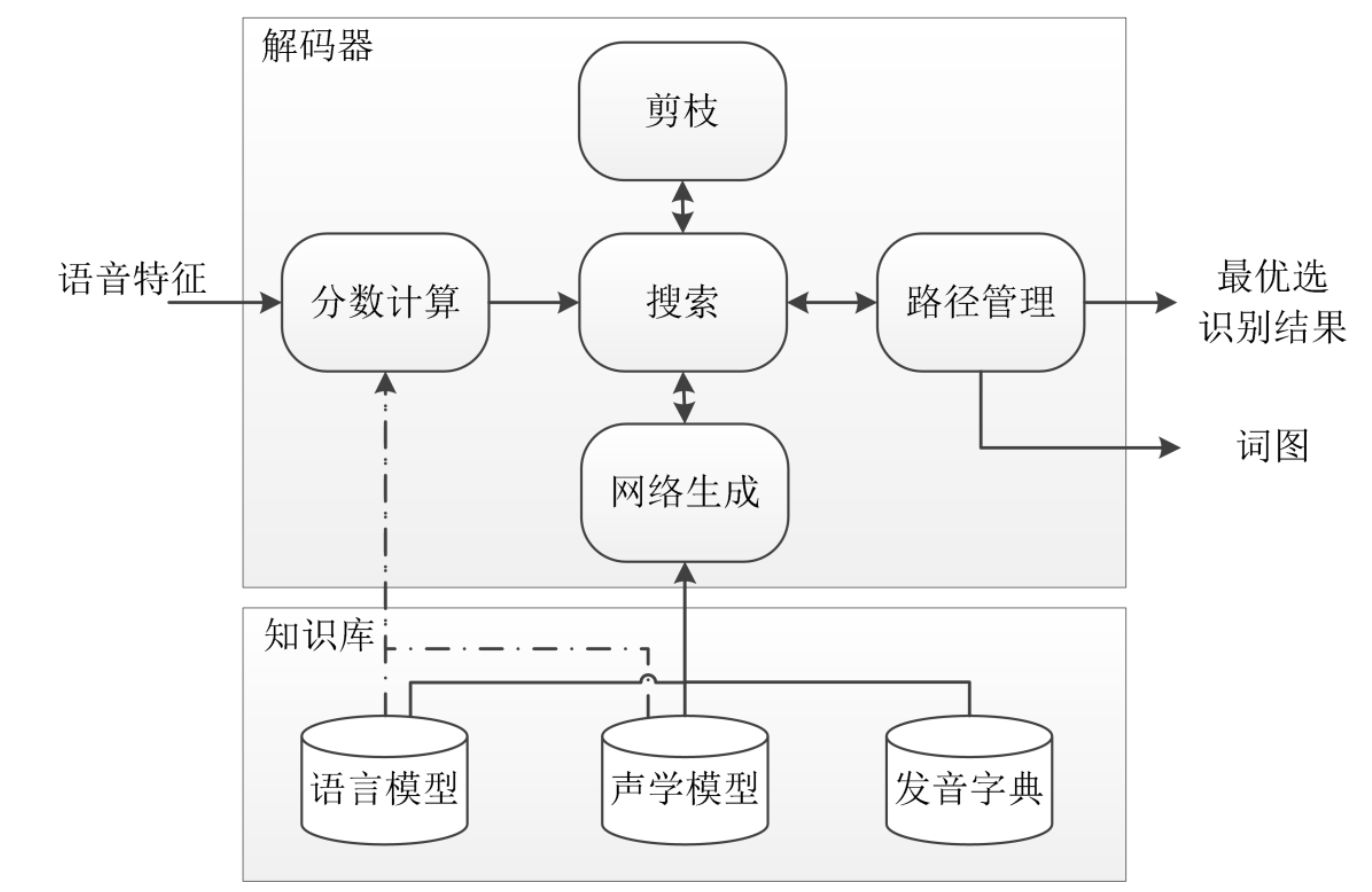
\includegraphics[clip=true, width=.9\textwidth]{figure/dec_arch.png}
    \bicaption[fig:dec_arch]{}{通用解码器架构}{Fig}{General Architecture of ASR Decoder}
\end{figure}


\subsubsection{基于加权有限状态机的网络生成算法}

网络生成模块主要负责构建解码搜索空间。搜索空间(也称为解码网络)通常与音素HMM或HMM状态连接,从语言模型,发音词典,声学模型和其他相关知识源编译。大词汇量连续语音信号解码网络的识别系统由各种知识源组成,形成搜索空间,一般可分为动态构造的解码网络和静态网络。基于动态网络解码器,前缀树发音字典用作搜索网络。语言模型通过动态查询将得分引入解码过程,然后通过重新输入字典树或字典树副本来搜索整个解码网络~\cite{young2002htk}。
动态网络解码器主要优势在于,由于字典和语言模型是分离,其占用内存极少,这个特点在以往移动网络技术和硬件技术不发达的时代,尤其是在嵌入式设备上内置解码器的时代,占有着绝对优势。但是动态网络的缺点是它解码速度较慢,时间复杂度较高,这也使其愈加难以满足当前海量语音信号的识别请求。
随着移动互联网和嵌入式设备的普及以及云技术的发展,语音信号的识别应用已发展为仅在嵌入式设备上保持简单的前端,而识别系统仍保留在服务器云中。此时,反映了基于WFST的静态网络解码器的快速优势。较短的识别时间允许服务器每单位时间接受更多的识别任务,因此静态编译的解码网络更适合于大量语音信号识别任务。

在LVCSR任务中,解码网络通常非常大。因此,网络结构需要采用各种手段来优化网络结构,并在不改变网络功能的情况下尽可能地减少网络中的节点和边数量。解码网络是解码器的基础,并确定在解码器的其他部分中应该使用哪种方法。在静态网络解码器中,解码网络不仅包含发音字典和声学模型,还包含完整的语言模型。语言模型状态和状态转换以有限状态机的形式合成到解码网络中,并且语言模型得分被存储为边上的状态转移概率。当解码时,仅通过累积整个路径状态转移概率可以获得语言模型得分。这类解码器的典型代表是基于加权有限状态转换器(WFST~\cite{mohri2002weighted}的解码器。

WFST最开始由AT\&T实验室Mohri和Riley等人在1997年引
入语音信号的识别领域。并且在理论上发展了确定化、最小化等一系列网络优化算法,为语音信号的识别的应用打好了理论基础。语音信号的识别各模型组件分别用如下方式进行WFST构建:

\begin{itemize}
\item N-gram语言模型在WFST中表示为G.根据N-gram语言模型的含义,它提供了单词历史的当前单词概率。语言模型需要具有记录最多N个单词的历史的信息。但是,当识别语音信号时(即,输入和输出是其符号集的单个元素),WFST应用程序不允许使用字符串输入和输出。因此,不可能在G构造过程的输入和输出上表达其历史,而是记录该状态的历史。另一个问题是N-gram模型的回退(Back-off),当语言模型训练语料未出现某一个N元词组的时候,就会以一个回退的(N-1)元模型概率乘以一个系数来替换。这部分表示为一个带有着权重但是输入为空的状态跳转边。

\item 字典在WFST中被表示为L。
字典实际上是发音规则的表示。最简单的方法是列出开始状态和结束状态之间每个单词的发音。同时,由于在与语言模型合成时连接了单词和单词,因此无法达到终止状态,并且需要将闭合边从终止状态连接到开始状态以形成闭环。针对字典的同发音问题,Mohri在文献~\cite{mohri2002weighted}中提出对于不同词的同发音发音
序列加入一组辅助符号,这样对于同发词语,其环路的输入符号序列就不再相同,可以确保字典的可确定化。

\item 上下文相关声学模在WFST中被表示为C。
一个上下文相关triphone模型一般表示为a-b+c,其中b是中心音素,
a和c为其前后上下文音素~\cite{seide2011conversational}。用WFST表示triphone模型实际上是在把三音素和单个音素之间进行对应,其输出就和发音字典的输入做相互对应,由此可以进行进一步合成。

\item 隐马尔可夫模型在WFST中被表示为H。
HMM模型天然具有多个的状态跳转特性,所以可以直接将其构建为多个WFST状态。隐马尔科夫模型的转移概率于是被转化为WFST的权重。而WFST输入是隐马尔科夫模型的状态索引,输出是该隐马尔科夫模型所表示的triphone建模单元。
\end{itemize}

当各个知识源WFST组件被构建完毕以后,可以利用WFST合成算法和优化算法将各组件最后进行合并和最终优化。如下:
\begin{equation}
HCLG = min(det(H \circ min(det(C \circ min(det(L \circ G))))))
\end{equation}

最终生成的WFST包含了所有的知识源,后文所讨论维特比搜索就在它上面进行。

\subsubsection{分数计算}

分数计算模块计算输入特征序列声学和语言分数,并将它们提供给搜索模块以供使用。应该计算哪个分数与解码网络结构和搜索算法有关。例如,在静态网络解码器中,语言模型得分已经被编译到解码网络中,因此只需要计算声学得分;对于动态网络解码器,除声学分数外,还需要计算语言模型分数。分数计算的研究主要集中在如何实现分数的快速计算。对于声学分数,通常执行以下三个方面:

\begin{itemize}
\item 硬件加速。利用 CPU 矢量计算器~\cite{kanthak2000using}
或者通用图形处理器(Graphics Processing Unit, GPU)~\cite{chong2009fully}
加速分数计算。这类方法通常来说不会带来计算误差(与硬件实现相关),所以对识别准确度没有影响。
\item 模型简化。采用复杂度更小、参数更少的分类器模型,或通过聚类和参数共享减
小模型复杂度。例如采用半连续 HMM~\cite{huang1990semi} 替代连续 HMM,以及传统的参数共享方式~\cite{young2002htk}亦属此类。这类算法一般都会带来识别准确度上面的损失,所以需要在
识别准确度、模型复杂度和计算速度之间做好一定的权衡。
\item 算法优化。 对声学分数的计算过程进行简化。这类方法一般是对声学分数进行近似计算,所以必然会带来一定识别准确度损失。一般而言, 衡量一个近似算法是否可用的标准是看其带来相对识别准确度损失是否可控制在5\%以内~\cite{cai2009efficient}。
\end{itemize}

对于语言分数计算,当采用 N 元文法模型时,通常从两个方面进行加速: 1)
减小每次查表操作上面的耗时,典型方法是采用最小完美哈希(Minimal Perfect Hash,
MPH)表实现语言模型的存储与查取~\cite{li2007fast,cardenal2002fast}; 2) 引入分数缓存~\cite{huijbregts2008fast}减少查表熵的次数。

\subsubsection{维特比搜索}

搜索模块负责在解码网络上搜索得到最优路径。不论是静态网络解码器还是动态网络解码器,目前都以令牌传递算法~\cite{young1989token}为主流的搜索算法。

令牌传递是维特比算法的另一个更通用和简单的实现。在算法中,每个HMM状态可以与令牌(Token)相关联,令牌存储令牌所经历的历史路径和路径得分直到当前帧。解码是根据状态转换(即,沿着解码网络的边)将令牌从解码网络的初始状态传递到终止状态的过程。每个帧令牌向前传递一次,同时传递令牌得分和路径信息,并在多个令牌同时传递到状态时进行令牌合并,仅保留具有最高得分的令牌。在处理完所有帧之后,获得最佳路径和最佳路径得分。

令牌传递算法的优点是可以方便地在令牌上保存其他信息以便在状态节点之间进行传递,从而实现更复杂解码过程,例如: 为了生成词图,在令牌合并后, 不是将次优令牌直接丢弃,而是作为其他候选路径保存于合并后的令牌之上。

\subsubsection{剪枝}

在LVCSR中,搜索空间太大而无法对整个解码网络执行完全搜索。剪枝用于消除解码过程中的低分数路径,从而减少计算量并确保不降低识别性能。根据解码器设计,剪枝可以应用于搜索的各个阶段(例如,开始或结束),或者可以应用于各种级别(例如,单词级别,音素级别,状态级别,令牌级别),但是可以归纳为两个基本类别:

\begin{itemize}
\item 束剪枝(Beam pruning) :束剪枝保留与最优路径分数较近的次优路径。
令 $v(t,j)$ 表示第 t 帧位于状态 j 最优路径分数,则第t 帧的最优路径分数为:
\begin{equation}
v_{max}(t)=max_s v(t,s)
\end{equation}

令 $f$ 为剪枝阈值(又称为束宽),则束剪枝只保留所有满足下式的路径:
$v(t,j)>v_{max}(t)\cdot f$
\item 直方图剪枝(Histogram pruning) :与束剪枝不同,直方图剪枝仅保留分
数最高 N 条路径, N 为设定剪枝阈值。之所以称为直方图剪枝是因为该方法
可以采用直方图统计高效地实现~\cite{pylkkonen2005new}。
\end{itemize}

\subsubsection{路径管理和词图}

路径管理模型主要作用是用于对搜索过程中得到的路径链表进行回溯,获取最优路径、
N-Best 结果和词图。同时,它也负责对剪枝过程中所剪掉的较差路径进行内存回收等操作。

\begin{figure}[!htp]
  \centering
    \captionstyle{\centering}
    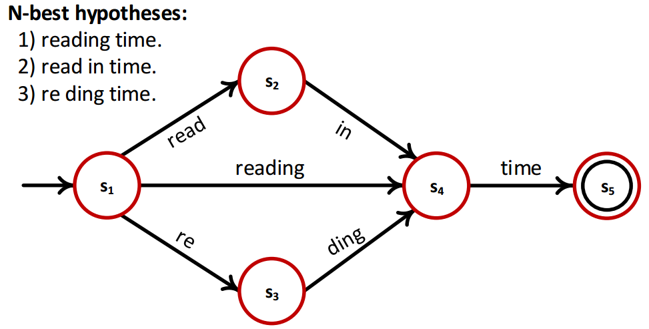
\includegraphics[clip=true, width=0.6\textwidth]{figure/lattice.png}
    \bicaption[fig:lattice]{}{N-Best候选序列和词图}{Fig}{N-Best Hypothesis and Lattices}
\end{figure}


由于N-Best候选序列中往往存在大量的公共部分(比如图~\ref{fig:lattice}中的“time”这个词),因此将公共部分优化在一起进行表示,也就是将多个候选序列转变成一张图来进行存储,将会更加紧致。在语音信号的识别中,这样一张图就称为词图。词图的生成所带来的额外消耗与生成N-Best候选序列类似。具体来说,其往往要求在解码过程中做令牌合并时,保留多个历史令牌记录。在记录完词图后,还需要词图剪枝步骤,其将冗余和无法连通边及其相应结点删去,得到最终比较紧致的词图。

词图具有较多用途(一些例子如图~\ref{fig:lattice-usage}所示),因此相较于N-Best候选序列,词图的处理往往是语音信号的识别系统中的一个标准模块。

\begin{figure}[!htp]
  \centering
    \captionstyle{\centering}
    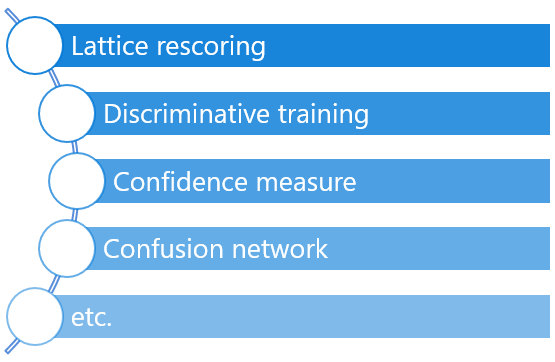
\includegraphics[clip=true, width=0.4\textwidth]{figure/lattice_usage.png}
    \bicaption[fig:lattice-usage]{}{词图用途举例}{Fig}{Applications of Lattices in ASR}
\end{figure}



\section{解码器研究中的待解决问题}
\label{chap:intro2-dec-future}

语音识别技术虽然相比多年以前已经有了长足的进步,但是在实际应用中还有很多困难需要处理。其中一个最主要难题就是语音识别推理搜索问题。
%
% 做什么事情
语音识别既是模式识别问题又是相应的推理搜索问题。前一个问题在数学上表示和描述了各种语音和语言现象,并且基于统计学习模式识别框架执行建模,该框架确定了语音识别系统可以实现的识别准确度的上限。在给定模型的情况下,后一问题研究如何使输入语音与模型匹配并推断最佳识别结果,其确定识别速度和实际可达到的识别准确度。在语音识别的推理搜索阶段,解码器功能组合声学模型以计算声学特征概率和语言模型计算的语言概率以获得最大概率词序列。
在语音识别推理搜索阶段,解码器是语音识别系统的核心和灵魂,所有信息都收集在这里。它将来自不同来源,不同层次和不同性质的知识和信息联系起来,以便它们相互补充并获得正确的语音识别结果。因此,如何有机地整合各种不同的信息是解码网络和解码算法设计中必须仔细研究和解决的问题。
从解码器功能的角度来说,它不仅是语音识别研究中各种理论,模型和算法的验证。
正确性和准确性的基本实验平台也是构建实际系统的基础所在。因此,在解码器的设计中必须平衡研究的便利性和工程的实际应用。


% 近来深度学习下发展现状和缺陷
近年来,深度学习模型被引入到语音识别声学和语言建模中以取代传统的分类器,显着提高了模式识别问题的准确性。基于深度学习语音识别,语音识别的推理搜索问题没有根本改变,因为它只是取代了分类器。
基于加权有限状态机(WFST)的推理搜索问题静态搜索空间构造技术~\cite{mohri2002weighted}和帧同步维特比(Viterbi)网络搜索算法~\cite{forney1973viterbi}是目前性能最好解决方案,但其仍存在一系列显著缺陷:
\begin{enumerate}
\item 该方案基于传统的混合高斯 - 隐马尔可夫模型(GMM-HMM)声学模型和N-gram语言模型。基于深度学习的声学模型和语言模型是最佳表现。研究还不充分,如何将新的声学和语言模型引入框架; 如何在提高推理搜索速度的同时充分利用模型性能; 如何基于多个知识源给出可靠的推理搜索置信度算法是一个亟待解决的问题。
\item 这种方案基于语音识别中每个知识源(声学,语言,语义等)的搜索空间的预构建和整体优化,产生巨大的搜索空间,包括离线构建,在线使用,动态修改和算法的其他方面。计算量和内存消耗量非常大,这是阻碍语音识别应用场景扩展的重要原因。为了解决这个问题,新的声学和语音模型的搜索空间整体优化是不够的,基于推理搜索中间状态的搜索空间动态优化研究几乎是空白。
\item 目前,语音识别系统基于多知识源建模结果,并对输入音频进行推理搜索。建模和推理搜索过程非常复杂,知识来源的划分依赖于强大的先验知识。大规模或非标记语音数据收集以及基于并行的深度学习技术使得构建直接模拟语音数据和文本序列的端到端模型及其相应的识别和推理搜索算法成为可能。当前的解码框架没有这种设计。
\end{enumerate}

因此,尽管基于深度学习模型,加权有限状态机和基于帧的维特比网络搜索算法的深度学习已经发展到基本可用水平,但是精度仍然不能满足人类之间的正常交流要求。速度限制也使得无法在低成本和低功耗的解决方案上工作,这些解决方案一起阻碍了语音识别技术的大规模商业应用。


\section{本章小结}
\label{chap:intro2-sum}


本章回顾了语音信号识别和推理搜索阶段的搜索和解码部分的基本内容和方法。解码器将由声学模型计算的声学特征概率与由语言模型计算的语言概率组合,以获得最大概率词序列。在语音信号的识别和推理搜索阶段,解码器是语音信号识别系统的核心和灵魂,并且在此收集所有信息。它将来自不同来源,不同层次和不同性质的知识和信息联系起来,使它们相互补充,得到正确语音信号的识别结果。因此,如何有机地整合各种不同的信息是在解码网络和解码算法的设计中必须仔细研究和解决的问题。
从解码器的作用来看,它不仅是验证语音信号识别中各种理论,模型和算法正确性的基本实验平台,也是构建实际系统的基础。因此,在解码器的设计中,还需要考虑研究的便利性和工程的实际应用。

本章中重点总结了目前解码器的研究现状及存在的缺点和实现难点。后续几章我们的改进工作将具体针对所有这些目前存在的问题进行展开。
